\documentclass[journal]{IEEEtran}
% IEEE Transactions on Industrial Informatics -- anonymous regular-paper draft
% Compile: latexmk -pdf main.tex
\usepackage{amsmath,amssymb,amsfonts}
\usepackage{algpseudocode}
% Local XeTeX/Tectonic builds: route IEEEtran's ptm (Times) family requests to
% the legacy Times Type1 faces so metrics match the pdfLaTeX reference build;
% the latexmk -pdf (pdfLaTeX) path is unaffected.
\usepackage{iftex}
\ifxetex
  \DeclareFontFamily{TU}{ptm}{}
  \DeclareFontShape{TU}{ptm}{m}{n}{<->ptmr8t}{}
  \DeclareFontShape{TU}{ptm}{b}{n}{<->ptmb8t}{}
  \DeclareFontShape{TU}{ptm}{m}{it}{<->ptmri8t}{}
  \DeclareFontShape{TU}{ptm}{b}{it}{<->ptmbi8t}{}
  \DeclareFontShape{TU}{ptm}{m}{sl}{<->ptmro8t}{}
  \DeclareFontShape{TU}{ptm}{m}{sc}{<->ptmr8t}{}
\fi
\usepackage{graphicx}
\usepackage{booktabs}
\usepackage{tabularx}
\usepackage{array}
\usepackage[table]{xcolor}
\usepackage{stfloats}
\usepackage{placeins}
\usepackage{url}
\urlstyle{same}
% Cross-references and citations. The cite package renders IEEE-style citation
% groups ([14]--[16], [20], [21]) with hyperref support.
\usepackage{cite}
\usepackage[colorlinks=true,linkcolor=black,citecolor=black,urlcolor=black]{hyperref}
\hypersetup{bookmarksnumbered=true,
  pdftitle={AgentWorkShop: A Modular Framework for Industrial Agent Integration},
  pdfauthor={},
  pdfsubject={IEEE Transactions on Industrial Informatics},
  pdfkeywords={industrial informatics, industrial agents, multi-agent systems, production system integration, semantic data integration}}

% Float placement only; IEEEtran margins and body type remain unchanged.
\setcounter{topnumber}{4}
\setcounter{bottomnumber}{3}
\setcounter{totalnumber}{7}
\setcounter{dbltopnumber}{2}
\renewcommand{\topfraction}{0.95}
\renewcommand{\bottomfraction}{0.80}
\renewcommand{\textfraction}{0.03}
\renewcommand{\floatpagefraction}{0.72}
\renewcommand{\dbltopfraction}{0.95}
\renewcommand{\dblfloatpagefraction}{0.72}

% Tight but conventional float separation; body type and margins are unchanged.
\setlength{\textfloatsep}{8pt plus 2pt minus 3pt}
\setlength{\dbltextfloatsep}{8pt plus 2pt minus 3pt}
\setlength{\intextsep}{7pt plus 2pt minus 3pt}
\setlength{\abovecaptionskip}{3pt plus 1pt minus 1pt}
\setlength{\belowcaptionskip}{2pt plus 1pt minus 1pt}

% Evidence snapshot: one archived integrated run with raw reports, run
% manifest, scenario definitions, and metrics.
% The two live engine-task logs are original outputs saved at execution time,
% as confirmed by the author; the structured run report retains their checked
% outcomes. The four-arm ablation has its own companion run record.
\newcommand{\resSeed}{42}
\newcommand{\resPhases}{20}
\newcommand{\resChecksTotal}{83}
\newcommand{\resChecksPass}{83}
\newcommand{\resChecksWarn}{0}
\newcommand{\resChecksFail}{0}
\newcommand{\resTotalWall}{26\,min}
\newcommand{\resDaqSamples}{55}
\newcommand{\resWriteP}{29.954\,ms}
\newcommand{\resTcpP}{47.8\,ms}
\newcommand{\resOpcP}{19.8\,ms}
\newcommand{\resMqttP}{19.3\,ms}
\newcommand{\resHttpP}{32.9\,ms}
% p95 per protocol line, same run: ~6 writes each. Recorded in the archive's
% metrics.csv (write_p95_ms) but reported in the body only since the 2026-10-12
% revision, so they live here rather than inline. Names must be letters only:
% \resTcpP95 would parse as \resTcpP followed by the characters "95".
\newcommand{\resTcpTail}{248.9\,ms}
\newcommand{\resOpcTail}{20.5\,ms}
\newcommand{\resMqttTail}{20.1\,ms}
\newcommand{\resHttpTail}{44.6\,ms}
% cross-protocol ranges over the four write families (min p50 = MQTT, max
% p50 = Modbus TCP; min p95 = MQTT, max p95 = Modbus TCP)
\newcommand{\resPfiftyRange}{19.3--47.8\,ms}
\newcommand{\resPninetyfiveRange}{20.1--248.9\,ms}
\newcommand{\resWriteNperLine}{6}
\newcommand{\resAblationRun}{\texttt{20260921181234-e1lite}}
\newcommand{\resFullIntercept}{18/18}
\newcommand{\resNoInterlockIntercept}{12/18}
\newcommand{\resNoReadbackIntercept}{18/18}
\newcommand{\resUngatedIntercept}{12/18}
\newcommand{\resBackstop}{130.2\,s}
% 134.7 s: defined but NOT used in the body (the drill's archived timing is
% 130.196 s, = \resBackstop); kept only so the symbol is not silently reused.
\newcommand{\resBackstopDrill}{134.7\,s}
\newcommand{\resPortFfive}{9/9}
\newcommand{\resPortCode}{0}
\newcommand{\resParamChecks}{4/4}
\newcommand{\resHitlLatency}{461\,ms}
\newcommand{\resMissionFrom}{200}
\newcommand{\resMissionTo}{204.704}
\newcommand{\resMissionPv}{204.70}
\newcommand{\resMissionTarget}{$204.704\pm0.75$}
\newcommand{\resBiaxSp}{30}
\newcommand{\resBiaxDaq}{19}
\newcommand{\resBiaxWrites}{3}
\newcommand{\resBiaxStart}{28.10}
\newcommand{\resBiaxFinal}{25.66}
\newcommand{\resBiaxTarget}{25.0}
\newcommand{\resBiaxTol}{0.7}
\newcommand{\resLlmWall}{156.3\,s}
\newcommand{\resGoalWall}{637.3\,s}
\newcommand{\resGoalFinal}{51.7}
\newcommand{\resJstar}{89.894}
\newcommand{\resJzero}{67.2}
\newcommand{\resControllerMin}{0.965}
\newcommand{\resControllerMean}{0.969}
\newcommand{\resControllerMax}{0.972}
\newcommand{\resInjStart}{31.25}
\newcommand{\resInjFinal}{32.17}
\newcommand{\resInjWrites}{2}
\newcommand{\resInjWall}{26.48\,s}
\newcommand{\resWwtpStart}{0.21}
\newcommand{\resWwtpFinal}{3.50}
\newcommand{\resWwtpWrites}{15}
\newcommand{\resWwtpWall}{169.27\,s}
\newcommand{\resWwtpCostStart}{181.5}
\newcommand{\resWwtpCostFinal}{179.1}
\newcommand{\resAnnealStart}{134.52}
\newcommand{\resAnnealFinal}{100.08}
\newcommand{\resAnnealWrites}{5}
\newcommand{\resAnnealWall}{102.76\,s}
\newcommand{\resAnnealSpeedFinal}{164}
\newcommand{\resAnnealSpeedTried}{176}
\newcommand{\resAnnealGain}{17.1\%}
% writeLockSeconds: node field default 30 s, constructor default 60 s; the
% online path enforces max(60 s, configured), so 60 s is the effective floor
% (unused in body since the pacing-window rewrite; kept for reference).
\newcommand{\resWriteLock}{60\,s}

% October 2026 deployment-scale campaign (v0.7.57), added with the revision.
% The hardened-pipeline run is archived at 91/91; three consecutive
% full-suite runs score 79/79 each (237 total; an earlier 80-per-run tally
% counted one S7 report assertion that is not a logged check). Per-run
% reports, manifests, and timelines are archived with each benchmark run.
\newcommand{\resPipeRun}{\texttt{benchmark-20261008045434}}
\newcommand{\resPipeTotal}{91}
\newcommand{\resPipeApi}{54}
\newcommand{\resCampaignRuns}{three consecutive}
\newcommand{\resCampaignTotal}{237}
\newcommand{\resCampaignApi}{45}
\newcommand{\resLoopTotal}{53}
\newcommand{\resAckTotal}{34}
\newcommand{\resDocsTotal}{91}
\newcommand{\resLinesLive}{34}
\newcommand{\resLinesRunning}{17}
% channel count across the three October 9 regression runs: 111/111/113;
% the body reports the range rather than one run's value.
\newcommand{\resChannelsLive}{111--113}
\newcommand{\resDaqOnline}{67}
\newcommand{\resWriteNodesLive}{77}
\newcommand{\resRecipesLive}{52}
\newcommand{\resBindingsLive}{385}
% approval->dispatch spans both campaigns: 8/9/9 ms (Oct 7-8), 9/6/6 ms (Oct 9).
\newcommand{\resHitlDispatchMs}{6--9\,ms}
\newcommand{\resLadderFrom}{66}
\newcommand{\resLadderTo}{63}
\newcommand{\resConsistencyErr}{0.0\,bar}
\newcommand{\resObsVerifyFast}{25.1\,s}
% 245.204 s (benchmark-20261007194413) / 245.184 s (-07194925), exact values
\newcommand{\resObsVerifyCadence}{245.20/245.18\,s}
\newcommand{\resCadenceWait}{218\,s}
\newcommand{\resWideRows}{869}

% October 9, 2026 regression campaign (v0.7.57), same live instance.
% Three runs archived at 92/92, 90/90, and 90/90; timeline.jsonl per run
% (S4/S5 process records, HITL card events).
\newcommand{\resNovRuns}{\texttt{benchmark-20261009021149}/\texttt{-024141}/\texttt{-033810}}
\newcommand{\resNovTotal}{272}
\newcommand{\resNovApi}{54}
\newcommand{\resNovDeadband}{0.15\,g}
\newcommand{\resNovZigzagFrom}{64}
\newcommand{\resNovZigzagTo}{63}
\newcommand{\resNovCorrFrom}{63}
\newcommand{\resNovCorrTo}{65}
\newcommand{\resNovWeights}{$32.49/32.33/32.22$\,g}
\newcommand{\resNovCadenceReject}{69\,s}
\newcommand{\resNovCardId}{\texttt{ap-2950a5b6}}
\newcommand{\resNovRunId}{\texttt{rr-51b0a0ac}}
\newcommand{\resNovScheme}{hold-pressure micro-up (sensitivity excitation step)}
\newcommand{\resNovSlope}{0.052\,g/bar}
% Oct 9 diagnostics: three-run distribution, not the single worst run.
% runs 021149/024141/033810: rows 663/843/861, in-spec 100.0/96.4/94.0%,
% std 0.042/0.186/0.237 g. \resNovInspec/\resNovWideRows/\resNovStd are the
% single third-run values; the ranges above are defined for reference and
% \resRowsRange is the one used in the body.
\newcommand{\resNovInspecRange}{94.0--100.0\%}
\newcommand{\resNovStdRange}{0.04--0.24\,g}
\newcommand{\resRowsRange}{663--869}
\newcommand{\resNovInspec}{94.0\%}
\newcommand{\resNovWideRows}{861}
\newcommand{\resNovStd}{0.24\,g}

% Seven-leg fault-suite outcomes (hardening ack-gate suite,
% tmp-e2e/hardening-ack-gate.mjs; archived in
% docs/audit/2026-10-08-production-hardening-report.md): 2 parameters
% promoted transport-acknowledged -> readback-verified by post-write
% re-read; 1 failed (broker unreachable, healthy sibling verified);
% 1 unverified (publish-only endpoint, three verification attempts).
\newcommand{\resAckPromoted}{2}
\newcommand{\resAckFailed}{1}
\newcommand{\resAckUnverified}{1}


\newcommand{\system}{the platform}

\begin{document}
\bstctlcite{IEEEbstctl}

\title{AgentWorkShop: A Modular Framework for Industrial Agent Integration}

\author{}
\markboth{IEEE Transactions on Industrial Informatics, Submitted Manuscript}{AgentWorkShop: Industrial Agent Integration}

\maketitle

\begin{abstract}
Industrial-agent applications must connect collaborative tasks to production
context, equipment interfaces, and process observations. AgentWorkShop is a
modular software framework that combines workspace and task services,
registered agent-harness adapters, scene configuration,
line--product--recipe--run context, semantic acquisition and control nodes,
protocol drivers, and analysis and modeling services. A task turn assembles
prompt context and scoped tools; a shared dispatcher checks each returned
operation before routing it to a handler. Industrial handlers apply
route-specific live-state checks, and owning services retain available
command, approval, observation, and recipe-version records. We evaluate two
implemented simulator paths in cast-film and annealing scenes. The
application-level path tests protocol access, readback, data lineage, and
model-gate enforcement; both model candidates fail the configured gates. Six
sequential tasks through one registered harness exercise bounded recipe
trials, synthetic approval, verified command readback, task completion, and
one run-tagged sample per task. All six post-completion samples remain outside
their target bands. The evidence supports the tested software integration
paths, but does not measure configuration-reuse benefit, process convergence,
quality improvement, physical-plant transfer, or cross-harness portability.
\end{abstract}

\begin{IEEEkeywords}
Industrial agents, industrial communication, industrial informatics,
production systems, semantic data integration.
\end{IEEEkeywords}

\IEEEpeerreviewmaketitle

\section{Introduction}
\IEEEPARstart{I}{ndustrial-agent} deployments must connect each task to its
production context, process signals, and equipment interfaces. Existing work
addresses end-to-end automation control, operator-reviewed control-sequence
generation, modular factory skills, and production scheduling
\cite{xia2025control,huang2026made,koehle2026llmdriven,waseem2026pretrained}.
Other studies target PLC code generation, context-aware control, resource
capability discovery, shop-floor coordination, digital-twin fault handling,
natural-language machine access, and robotic-line control
\cite{liu2026agents4plc,wu2025instructmpc,lim2025llmenabled,zhao2026shopfloor,gill2025llmdt,hofmann2025nlc}.
Across production lines, agent roles, signal maps, protocols, objectives, and
product/run context vary. A reusable framework must configure these
differences around shared task and operation services while keeping each
action tied to its active production context.

Consider two production scenes with different process signals and interfaces:
cast-film thickness control and annealing-zone temperature control. An agent
task in either scene needs production context, typed signal access, and a
route from a named operation to the configured device protocol. The framework
must also distinguish a command receipt from a subsequent process
observation. The shared task and operation services can therefore be
configured with scene-specific signal maps, protocols, and limits while
retaining a common execution path. In this paper, the two simulator scenes
demonstrate that configured composition; they do not measure the effort or
benefit of changing configurations.

This paper presents AgentWorkShop, a configurable industrial-agent framework
that connects collaborative tasks and registered harnesses to production
context, manufacturing execution system (MES) data, analysis and modeling
services, data-acquisition (DAQ) and write-control (DCW) nodes, and
protocol-specific drivers. Its access surfaces include command-line, web,
SDK, REST, MCP, and A2A interfaces. Task and chat routes enter the
collaboration runtime, whereas a direct REST tool-invocation route can call
the shared operation dispatcher without creating a task.
Scene blueprints define signal maps, objectives, and guards; channel profiles,
tool policies, and agent bindings scope operations. Agents and callers invoke
named operations through shared runtime checks; the framework does not choose
routes autonomously and retains proposals, command confirmation, and process
observations as distinct records. Fig.~\ref{fig:arch} presents the system
architecture, and Fig.~\ref{fig:runtime} shows the cross-module task flow.
Section~IV details the node-exploration and recipe lifecycles.

The paper makes three contributions:
\begin{enumerate}
\item It defines a cross-layer task-to-operation contract that resolves
  production context before an agent turn, rechecks each returned operation
  at a shared dispatcher, routes semantic process nodes to configured device
  drivers, and links command receipts separately from process observations.
\item It implements this contract through replaceable harness adapters,
  scene and production-context configuration, analysis and modeling
  services, semantic device access, and route-specific command and recipe
  lifecycles. The contribution is this composition and evidence boundary;
  it does not introduce a new agent-reasoning or process-control algorithm.
\item It evaluates two current-version simulator paths across cast-film and
  annealing configurations. The application-level run verifies protocol
  reads, bounded writes, readback, and data lineage, while both model
  candidates fail the configured gates. Six sequential tasks through one
  registered harness record bounded recipe trials, synthetic approval,
  verified readback, task completion, and run-tagged samples; all samples
  remain outside their target bands. The evidence supports these tested
  integration paths, but does not measure configuration-reuse benefit,
  successful process optimization, convergence, physical transfer, or
  cross-harness portability.
\end{enumerate}

Section~II reviews related industrial-agent and integration work.
Section~III presents the design rationale, architecture, and cross-module
execution flow; Section~IV explains module responsibilities and their
integrated operation. Section~V describes the experiments and results, and
Sections~VI and~VII discuss the evidence limits and conclude the paper.

\section{Related Work}
\label{sec:related}
This section relates AgentWorkShop to plant-facing industrial agents and to
production and automation abstractions for context, tool access, and
operational constraints. Table~\ref{tab:nearest} compares selected systems
that address control generation, factory-module coordination, MCP-based
resource access, semantic recipes, and supervisory service reconfiguration.
It uses execution scope, stated integration boundary, and evaluation focus as
common dimensions. This is a focused comparison rather than an exhaustive
survey, and it does not treat an unreported feature as absent.

\subsection{Industrial Agents and Plant Integration}
Industrial-agent systems span end-to-end automation control, supervisory
services, programmable logic controller (PLC) interfaces, manufacturing
coordination, and operator-facing machine access. Xia et al. present an
LLM-agent framework for end-to-end industrial automation control, using
structured prompts and event-driven context for production planning and
operation \cite{xia2025control}. Huang et al. present a multimodal
architecture whose stated focus is automated control generation for
industrial cyber-physical systems \cite{huang2026made}. Biskupovic et al.
study agent-based supervision for service-oriented industrial systems
\cite{biskupovic2025supervision};
Agents4PLC and InstructMPC address PLC code generation and human--LLM
context-aware control, respectively
\cite{liu2026agents4plc,wu2025instructmpc}. Manufacturing studies consider
dynamic resource-capability exploration \cite{lim2025llmenabled}, multi-agent
shop-floor coordination \cite{zhao2026shopfloor}, and digital-twin-supported
fault handling \cite{gill2025llmdt}. Natural-language machine access
\cite{hofmann2025nlc} and real-time LLM control of a robot-operated serial
line \cite{waseem2026pretrained} extend this work to operator interfaces and
robotic-line control. Together, these studies address different operational
contexts, interfaces, and allocations of responsibility between agents,
operators, and controllers.
\begin{table*}[!t]
\centering
\caption{Selected plant-facing agent systems and their integration settings.
The table compares the stated execution scope and evaluation focus; it is not
a performance ranking and does not infer unreported features.}
\label{tab:nearest}
\small
\setlength{\tabcolsep}{4pt}
\begin{tabularx}{\textwidth}{@{}p{2.3cm}p{2.5cm}XX@{}}
\toprule
System & Execution unit & Stated integration boundary & Evaluation focus \\
\midrule
Huang et al. \cite{huang2026made} & Automated industrial control generation & Multimodal industrial CPS architecture; the paper's stated focus is generating control actions & Control generation is its stated scope; no head-to-head comparison is made here \\
K{\"o}hle et al. \cite{koehle2026llmdriven} & Factory modules; orchestrator, peer-to-peer, and monolithic designs & Per-module MCP servers expose OPC UA methods, with MQTT coordination, injected factory state, and state-based tool filtering & Nine simulated production challenges, including silent-fault detection \\
Vieira da Silva et al. \cite{silva2025mcpmanufacturing} & LLM planning and execution of manufacturing steps & Manufacturing resource functions exposed through MCP & Laboratory-scale multi-step process with constraint handling \\
K{\"o}hle et al. \cite{koehle2025semanticrecipes} & AI-assisted production-recipe composition & Reusable semantic recipes composed from OPC UA skills and validated by virtual commissioning & Proof-of-concept assembly workstation represented in Unity \\
Biskupovic et al. \cite{biskupovic2025supervision} & Service selection and reconfiguration in service-oriented ICPSs & Predefined component library; performance and computational-load criteria; online monitoring & Reselection after poor performance; reported adaptability and performance results \\
\midrule
AgentWorkShop (this work) & Collaboration task and registered harness call & Line--product--recipe--run context; per-call policy checks; semantic process nodes resolve to configured protocol drivers & Two configured simulator scenes exercise the task-to-device path; command receipts and process observations remain distinct, context-linked records \\
\bottomrule
\end{tabularx}
\end{table*}

These systems target complementary levels of the industrial-agent stack.
Vieira da Silva et al. expose manufacturing resource functions through MCP
and evaluate LLM-driven multi-step planning with constraints; K{\"o}hle et al.
compose reusable OPC UA skills into semantic recipes and validate them through
virtual commissioning \cite{silva2025mcpmanufacturing,koehle2025semanticrecipes}.
K{\"o}hle et al. also examine MCP-based coordination across factory modules,
while Huang et al. focus on control generation and Biskupovic et al. on
service reconfiguration \cite{koehle2026llmdriven,huang2026made,biskupovic2025supervision}.
AgentWorkShop instead describes a modular task-to-operation integration path
that combines production-context binding, per-call checks, semantic
node-to-driver routing, and distinct command and process records. These are
scope dimensions, not claims that prior work lacks any one mechanism. With no
head-to-head experiment, the contribution is the implemented composition and
evidence boundary, not comparative advantage or a new reasoning/control
algorithm. Agent strategy remains replaceable.
Authority and command confirmation are operational services consistent with
safety-aware decision support \cite{jiang2026agentic}; they do not replace
process protection or establish operator effectiveness.

\subsection{Production Context, Agent Interfaces, and Automation}
Industrial integration also depends on abstractions that are not specific to
agent architectures. MCP standardizes tool discovery and calls with
request-scoped authorization \cite{mcp2024}, whereas
ISA-88 and ISA-95 describe recipes and production operations
\cite{isa88_2010,isa95_2025}. Run-to-run methods connect process observations
to successive production runs \cite{moyne2000r2r}. At the agent level,
AgentSpec and CaMeL address tool behavior and capability-based information
flow \cite{wang2025agentspec,debenedetti2025camel}. Together, these works
provide complementary abstractions for production context, tool interaction,
and information flow. AgentWorkShop composes such abstractions with its task
runtime, operation checks, semantic I/O, and route-specific records; this
paper evaluates selected paths through that composition rather than proposing
a replacement for the underlying standards.

Industrial security and record requirements further constrain that
architecture: FDA guidance discusses trustworthy records and audit trails
\cite{part11}, IEC~62443-3-3 specifies system-security requirements
\cite{iec62443-3-3}, and DNP3 includes select-before-operate
\cite{ieee1815dnp3}. Control-assurance methods address state evolution through
shielding, control-barrier functions, or Simplex architectures
\cite{alshiekh2018shielding,ames2017cbf,sha2001simplex}. These standards and
methods inform the boundaries within which an industrial-agent framework must
operate; they are not contributions claimed by AgentWorkShop.

The evaluation tests selected software paths and simulator scenes, not
physical-plant performance.

\begin{figure*}[!t]
\centering
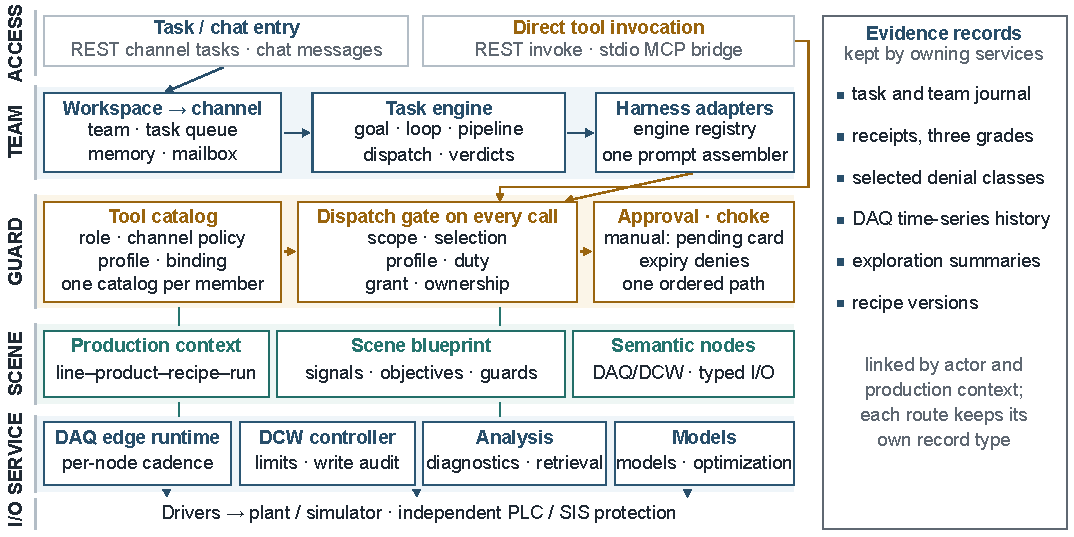
\includegraphics[width=\textwidth]{resources/fig-architecture-2026-9pt.pdf}
\caption{AgentWorkShop software architecture. Access, collaboration,
governance, production context, services, and field I/O form six connected
bands. Registered harness and driver interfaces expose extension points;
route-specific records remain in their owning services and are linked by
actor and production context. The field interface ends at the registered
drivers; PLC and safety-instrumented protection remain external.}
\label{fig:arch}
\end{figure*}
\section{System Design}
\label{sec:design}
AgentWorkShop is designed for industrial tasks whose agents, production
contexts, interfaces, and process signals vary between deployments. A useful
framework must let these differences be configured without changing the
shared task runtime, while ensuring that a proposed operation is checked
against the active production context before it reaches a device. It must also
retain enough route-specific evidence to distinguish a returned command
receipt from a measured process response.

\subsection{Design Rationale and Requirements}
\label{sec:principles}
Five requirements---scene variability, harness variability, operation
authority, outcome observability, and extensibility---organize six design
rules (D1--D6). These are deployment constraints drawn from the target
workflows. D1 stores scene settings as versioned data;
D2 provides registered harness, tool, and driver interfaces; D3 separates
proposal from execution; D4 treats the tool catalog as discovery rather than
permission; D5 routes actuator writes through the common DCW admission point;
and D6 retains evidence by operation.

The requirements trace to implementation and evaluation as follows.
Scene variability maps to D1, scene blueprints, and context resolution;
harness variability and extensibility map to D2, the registered harness and
driver interfaces; operation authority maps to D3--D5, the shared dispatcher,
grants, bindings, and write admission; outcome observability maps to D6,
route-specific receipts, and observations. In the evaluation, R13 exercises
two scene-specific protocol and data paths; R20 exercises the configured
task-to-device path through one registered harness, synthetic approvals, and
route-specific records. These tests do not isolate profile or binding changes
under matched conditions, establish third-party extension or cross-harness
portability, or show target attainment in R20. Older scripted and regression
records are retained in the companion evidence package, but do not support
the current integration claims. AgentWorkShop supplies task and operation
services; agent strategy and independent process protection remain outside
this design.

\subsection{Layered Architecture}
\label{sec:layers}
\label{sec:arch}
Fig.~\ref{fig:arch} maps the reference implementation onto six bands and
their route-specific evidence records. The access band exposes command-line,
web, SDK, REST, MCP, and A2A entry surfaces. Task and chat routes enter the
collaboration band, which contains workspaces, channels, task queues, shared
memory, mailboxes, task templates, and harness adapters. A direct REST
tool-invocation route can call the shared operation dispatcher without
creating a task or invoking a harness; MCP also includes separate management
and task operations. The governance band projects an operation catalog and
checks each invocation. The context band assembles bound-line and active-run
information for prompt grounding, while operation handlers resolve the live
state relevant to their route. The service band provides acquisition, write
control, analysis, retrieval, and optional model services. The field-I/O band
resolves semantic nodes to built-in or plugin drivers for a plant or
simulator.

Each band has a distinct responsibility. Task/chat routes enter the task
runtime; direct operation routes enter the dispatcher; and both use shared
operation checks where applicable. A harness adapter supplies
agent-specific interaction on task paths, semantic nodes hide protocol
details from operations, and the driver registry provides the device-facing
extension point. Owning services retain task, command, observation, and
version records separately and link them to available actor and production
context. No single status conflates these outcomes.

\subsection{Cross-Module Execution Flow}
\label{sec:executionflow}
Fig.~\ref{fig:runtime} summarizes a task turn from entry through operation
execution, with route-specific evidence retained by owning services. The
runtime assembles prompt-time production context and a scoped tool catalog
before invoking a registered harness. This context is grounding information
refreshed on each agent turn, not a task-pinned transaction. For
each returned tool call, the shared dispatcher rechecks invocation scope
and channel policy; industrial operations also receive current grant and
binding checks before handler selection. The selected handler applies its
own route-specific guards, approval, revalidation, and device-I/O steps.
Command receipts and any later process observations remain distinct records.

For an industrial operation $u$ by agent $a$ in channel $c$, define the
shared dispatch condition as
\begin{equation}
\mathcal{A}(a,c,u)=S(a,c,u)\land P(c,u)\land G(a,u)\land B(a,u),
\label{eq:dispatch-contract}
\end{equation}
where $S$, $P$, $G$, and $B$ denote invocation scope, current channel policy,
runtime grant, and agent binding/resource ownership, as applicable to the
operation. The policy term includes
the applicable channel tool selection, profile, and duty-separation checks.
This condition is necessary for handler selection, not sufficient for
actuation: the selected route applies its own guards and approval, then
rechecks authority and applicable limits before dispatch.

Fig.~\ref{fig:execution} gives pseudocode for these cross-module contracts;
it is a reference flow rather than one literal orchestrator function.
Route-specific timing, approval, and evidence rules are detailed in
Section~\ref{sec:modules}.

\begin{figure*}[!t]
\centering
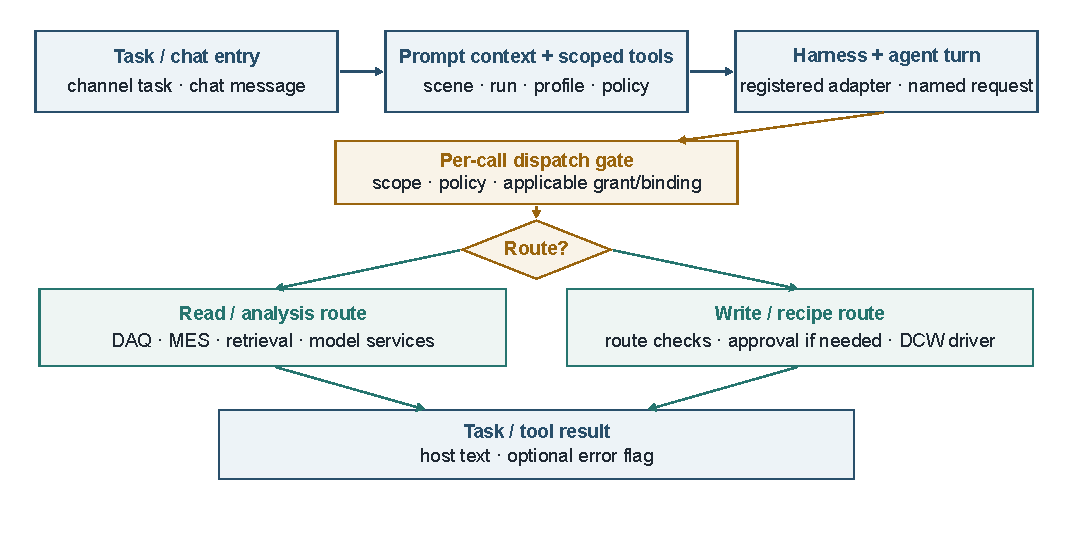
\includegraphics[width=\textwidth]{resources/fig-runtime-2026-9pt.pdf}
\caption{Cross-module task execution in AgentWorkShop. The task path assembles
a channel-scoped tool catalog and per-turn prompt context. Each returned call
is rechecked for scope and policy; the handler resolves applicable live state,
including grant, binding, and active-run checks on recipe operations. The
shared tool result contains host text and an optional error flag; route
records remain with owning services. The prompt-time context is not passed as
a transactional authorization token. Dispatch-gate errors return before
handler execution, whereas route-specific handlers may read state before
refusing a write. Durable denial auditing is selective. Receipts and later
observations remain distinct.}
\label{fig:runtime}
\end{figure*}

\begin{figure}[!t]
\centering
\begin{algorithmic}[1]
\Require task $q$, channel $c$, bound agent $a$
\Ensure task result; any retained evidence remains with its owning service
\State $x_t \gets \Call{ResolvePromptContext}{c,q}$
\State $T \gets \Call{FilterToolCatalog}{a,c}$
\State $m \gets \Call{RetrieveMemory}{q}$
\State $p \gets \Call{AssemblePrompt}{q,x_t,m}$
\State $h \gets \Call{InvokeRegisteredHarness}{a,p,T}$
\ForAll{tool request $u$ returned by $h$}
  \State $g \gets \Call{CheckScopeAndChannelPolicy}{a,c,u}$
  \If{\textbf{not} $g$}
    \State \Call{ReturnToolError}{h,u}; \textbf{continue}
  \EndIf
  \If{$u$ is an industrial operation}
    \State $v \gets \Call{CheckGrantBindingOwnership}{a,u}$
    \If{\textbf{not} $v$}
      \State \Call{ReturnToolError}{h,u}; \textbf{continue}
    \EndIf
  \EndIf
  \State $k \gets \Call{SelectHandler}{u}$
  \State $r \gets \Call{ExecuteRouteHandler}{k,a,c,u}$
  \Comment{handler resolves live state and may persist route-specific records}
  \State \Call{ReturnDeclaredToolResult}{h,r}
\EndFor
\State \Return task state and tool results
\end{algorithmic}
\caption{Reference pseudocode for cross-module execution in AgentWorkShop.
Evidence persistence is route-specific and remains with the owning service;
the shared tool result does not carry a generic evidence envelope.}
\label{fig:execution}
\end{figure}

\section{Module Functions and Integration}
\label{sec:modules}
The architecture in Fig.~\ref{fig:arch} is implemented as cooperating
modules rather than a single monolithic agent. Shared interfaces connect
task execution to configuration, industrial services, protocol drivers, and
route-specific evidence. This section describes those responsibilities and
the checks that preserve their boundaries.

The extension contracts expose the data passed at each boundary. A harness
call is normalized as \texttt{HostToolCall(toolName, arguments)} and returns
\texttt{HostToolResult(text, isError)}. A DCW driver accepts an engineering
value, tolerance, range, and driver configuration; its result separates write
status, raw value, readback, and acknowledgment grade (readback-verified,
transport-ack, or unverified). Each DAQ sample stores its node, timestamp,
value, and state, with optional line, product, recipe, and run IDs. A write
anchor records line/node, prior and requested values, source, actor, time, and
optional run/task/approval IDs; recipe definitions retain separate versions.
These fields keep tool errors, device receipts, observations, and production
lineage inspectable as separate records.

\subsection{Task Runtime and Harness Adapters}
Task and chat access surfaces create or join a workspace channel, where the
task engine manages members, task queues, shared memory, and execution
templates. A direct REST tool-invocation endpoint can enter the shared
dispatcher without creating a task or invoking a harness; the stdio MCP
operation bridge uses this route, while other MCP operations expose management
and task services.
The harness registry instantiates an adapter behind a common agent interface;
the prompt builder combines the task with the active scene brief, industrial
context, channel profile, agent binding, and retrieved memory. Tool calls
return to the shared dispatcher regardless of which registered harness
produced them. The registry is an extension point; the experiments do not
establish portability across harnesses. Industrial context is assembled for
each agent turn rather than pinned for the task lifetime. Operation handlers
check current route-specific state at invocation; recipe writes recheck the
binding, authorization, and active run after any human-approval wait. The
implementation does not compare the complete prompt-time
line--product--recipe--run snapshot with a task-pinned context version, so the
prompt snapshot is grounding information, not a transactional authorization
token.

\subsection{Production Context and Configuration}
Scene blueprints describe devices, signal maps, objectives, and process
guards. A task resolves these definitions against its active
line--product--recipe--run context. The channel profile selects the available
capability family, the tool policy narrows the operation catalog, and the
agent binding scopes the nodes, controls, and recipe operations available to
that member. These filters can restrict one another but cannot broaden the
underlying device range. The dispatcher re-reads policy at execution, so a
cached catalog does not retain authority after a grant or policy change. The
prompt builder assembles the agent's available bound-line and active-run
context on each turn; it does not pin the complete context tuple to the task.
Specific production snapshot, trial, and MPC routes, together with Hybrid Twin
training submissions, resolve and validate a versioned \texttt{SceneContract}
at operation time. The Twin physics-specification draft route can instead
accept a caller-supplied scene description; SceneContract enforcement is
therefore route-specific and does not validate or pin all prompt context.

\subsection{Acquisition, Analysis, and Modeling Services}
Semantic DAQ nodes expose typed values, engineering units, ranges, and
sampling settings while hiding protocol-specific reads. A per-node DAQ
runtime schedules acquisition and stores timestamped observations; the
gateway aggregates node pipelines. MES-facing operations provide the
configured production-data path. Analysis and retrieval services consume
these records, while optional model, training, optimization, and digital-twin
services are invoked through their registered operation handlers. These
services complement the agent workflow; AgentWorkShop does not prescribe a
single optimization strategy.

\subsection{Semantic I/O and Actuation}
The driver registry resolves a semantic node to a built-in or plugin driver.
DAQ handlers use the node's acquisition interface; DCW handlers route a
write or readback through the controller and the configured protocol driver.
This separation lets recipes and agents refer to semantic controls without
embedding Modbus, OPC UA, MQTT, HTTP, or MES transport details in their
operation arguments. The supported driver mappings are implementation
interfaces; only the mappings and workflows enumerated in Section~\ref{sec:eval}
are experimentally exercised.

\subsection{Shared Dispatch and Write Admission}
\label{sec:governed}
Every named operation passes the dispatcher. Its ordered checks validate
invocation scope and current channel policy (tool selection, profile, and
applicable duty separation), then the agent's binding and runtime grant and
ownership of referenced resources.
A refusal returns the excluding condition. Denial persistence is selective:
grant denials and selected resource-reference denials have explicit audit
paths, whereas scope and channel-policy denials are not uniformly retained as
durable audit events. A catalog entry therefore describes availability but
does not authorize execution. Handlers
for operations that require manual approval suspend for a decision, then
revalidate authority and active limits before dispatch.

All actuator writes converge on the DCW admission point. For an online node
write, the admissible interval is
\begin{equation}
\mathcal{I}^{\mathrm{online}}_n(t)=\mathcal{H}_n\cap\mathcal{B}_n
\cap\mathcal{P}_n(t)\cap\mathcal{R}_n(t),
\label{eq:admission}
\end{equation}
where $\mathcal{H}_n$ is the hard engineering range and $\mathcal{B}_n$,
$\mathcal{P}_n$, and $\mathcal{R}_n$ are the baseline, active-product, and
active-recipe limits. Missing optional limits impose no restriction, whereas
an empty intersection rejects the request and identifies the excluding
layer. Recipe dispatch applies the hard, baseline, and product limits to the
replacement recipe rather than intersecting with the previous recipe window.
The actuator path also enforces step, interval, and hold-window checks.
These admission rules constrain commands; process objectives and coupled
variable guards are assessed from later observations. The framework does
not replace independent PLC or safety-instrumented protection.

\subsection{Integrated Operation and Route-Specific Evidence}
\label{sec:tasklifecycle}
A recipe trial illustrates how the modules cooperate. The task runtime
delivers a named \texttt{recipe\_trial} call from the agent harness; the
dispatcher checks the agent's recipe binding and execution scope; the recipe
handler checks the active run, candidate parameters, and route timing; and a
manual binding requests approval before the DCW controller sends the batch
through its driver. The handler returns a per-parameter receipt. The caller
then obtains DAQ observations and can request a separate update, apply, or
rollback operation. A trial receipt confirms command handling; it does not
by itself establish process attainment or persist a new recipe version.

The routes retain different records because they answer different
questions. A driver acknowledgment reports command evidence; DAQ reports a
process observation; an exploration summary records a bounded probe; and a
recipe version records a saved definition. Their relation through actor and
production context allows an execution to be inspected without treating
these outcomes as interchangeable.

\subsection{Route-Specific Lifecycles and Evidence}
\label{sec:routes}
\label{sec:mech}
\label{sec:objective}
\label{sec:nodeexec}
\label{sec:ack}

\paragraph{Timing and approval}
Timing guards are route-specific. Online node writes enforce an effective
minimum spacing of 60\,s. Recipe dispatch uses a per-recipe interval anchored
to approval, while trials also use a configurable per-line cadence (default
300\,s). The recipe interval can refuse a proposal before an approval request
is created. Checks occur at proposal or execution according to the operation,
and experiment-specific pacing overrides are reported with the corresponding
results.

Manual bindings create an approval request containing the actor, node or
recipe, candidate values, applicable limits, expiry, and parameter bases.
The default wait expires after 180\,s and refuses execution. After approval,
the executor rechecks authorization and active limits to account for context
changes during the wait. For \texttt{recipe\_apply}, a changed definition
requires a new proposal; an unchanged approval dispatches a copy of the
approved parameter snapshot. A line-level recipe mode defaults to manual;
changing it to automatic requires administrator confirmation. The approval
record authorizes a workflow action and does not replace process protection.

\begin{figure*}[!t]
\centering
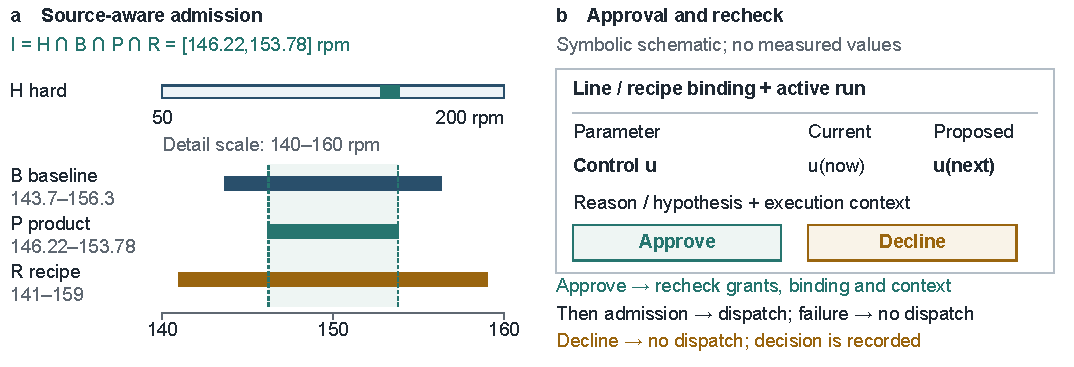
\includegraphics[width=\textwidth]{resources/fig-admission-hitl-2026.pdf}
\caption{Admission and approval boundaries. (a) Archived RPM example:
online node interventions use the four-layer value interval of
Eq.~(\ref{eq:admission}),
whereas recipe dispatch omits the prior recipe window. (b) Symbolic human
approval binds a proposed action and authority fields; execution checks run
again after approval, which does not reserve equipment state.}
\label{fig:hitl}
\end{figure*}

\paragraph{Node probe}
The bounded node probe is exposed as \texttt{optimization\_explore} to the
Auto Modeling Lab (AML) optimization profile (\texttt{aml\_optimization}).
The profile validates a bound control and target DAQ scope,
captures a starting control and target baseline, invokes the internal DCW
write path, then waits 10--300\,s (default 45\,s) and queries a trailing 45-s
target window before saving an exploration summary. Since each window is
relative to its query time, approval can separate baseline sampling from
actuation; a 10-s wait can leave about 35\,s of pre-write samples in the later
window. The command receipt and target summary are therefore returned
separately. A successful changed-value write opens a node-optimization
record; refusal or expired approval creates a rejected summary without a
post-write sample.

\paragraph{Recipe operations}
\texttt{recipe\_trial} checks the bound recipe and active run, then dispatches
candidate overrides as a batch with per-parameter verification. The caller
subsequently queries DAQ and decides whether to save a new definition with
\texttt{recipe\_update}, restore one with \texttt{recipe\_rollback}, or
dispatch a version with \texttt{recipe\_apply}. These steps are separate: a
trial does not save or apply a version, and endpoint verification is not a
process-response measurement. Public direct-node control is closed; the
bounded probe and recipe operations are the configured operation surfaces.
The historical four-scene results use an earlier direct-node path and do not
test current profile or binding adaptation across scenes.

\paragraph{Command verification}
Command confirmation and process response answer different questions. A
driver ACK is graded as \texttt{readback-verified}, \texttt{transport-ack},
or \texttt{unverified}. A matching endpoint read supports the first grade; a
transport or MES application receipt supports the second. Recipe batch
verification assigns \texttt{verified}, \texttt{unverified}, or
\texttt{failed}; if no matching readback is available, it attempts up to
three independent reads, 2\,s apart. A matching retry upgrades the final ACK,
while exhausted retries remain unverified. The initial ACK remains in write
history and the final ACK and verdict are retained with the batch.
Per-parameter receipts preserve successful outcomes when another parameter
fails. A readback-verified setpoint does not establish target attainment.

\paragraph{Observation, verdict, and compensation}
The caller performs recipe-path observation after batch dispatch. The October
recipe case therefore compares a recipe definition, endpoint readback, and
DAQ sample as separate representations. Saving a definition, applying it to
equipment, and observing its process response are separately evidenced
operations. The evaluation does not combine these route-specific records into
one universal end-to-end record.

An open node record provides a monitoring backstop. After 120\,s it polls
every 30\,s; three cumulative samples outside the recipe monitoring window
trigger a system-attributed rollback request toward the preceding value.
Missing samples do not count as breaches. A caller's \texttt{keep},
\texttt{rollback}, or \texttt{uncertain} verdict records its interpretation;
compensation is a new command subject to its applicable admission policy.
The write audit deduplicates the same value on the same node within 10\,s,
while batch receipts, exploration summaries, DAQ history, and recipe versions
retain their distinct lifecycles. Linking these records by actor and
production context allows the command, endpoint evidence, and process
observation to be inspected without treating them as interchangeable.
\label{sec:agentloop}


\FloatBarrier
\section{Experimental Evaluation}
\label{sec:eval}
The evaluation examines two bounded simulator paths. R13 is an exploratory
application-level protocol and data-path run; it supports only the recorded
protocol, readback, lineage, and model-gate outcomes because its exact runtime
source was not pinned. R20 is the primary current-version result: six
sequential tasks through one registered harness across two configured scenes,
with a run-specific source reconstruction kit. It supports the tested
task-to-device integration path, not configuration-reuse benefit or process
attainment. All process experiments use repository simulators. Older
scripted and regression records remain in the companion evidence package and
are not pooled with these results.

\subsection{Evidence Units and Experimental Procedure}
\label{sec:testbed}
\label{sec:procedure}
R13 uses two configured protocol/data paths in cast-film and annealing
simulators. R20 uses the registered \texttt{omp} harness in those scenes, with
three sequential task executions per scene on one simulator instance per
scene. The companion reproducibility package records the older protocol,
controller, deployment, direct-node, and scripted-recipe cases separately;
they are not part of the current primary result.

\subsection{Current-Version Two-Scene Simulator Integration}
\label{sec:crossscene}
An exploratory v0.8.0 application run used the cast-film and annealing
simulator presets. Five protocol families---OPC UA, MQTT, Modbus TCP, Modbus
RTU over TCP, and HTTP/REST---passed read probes; bounded writes returned
matching readbacks. Six 120-s runs per scene at 1-s sampling produced
lineage-verified datasets.

For each dataset row $i$, let $m_i$ be the last MV value in its history window
and $c_i$ the first CV value in its target horizon. The gate computes
\begin{equation}
r_{\Delta}(\ell)=\operatorname{corr}(\Delta m_i,\Delta c_{i+\ell}),
\qquad \ell\in\{1,2,3\},
\label{eq:r13corr}
\end{equation}
using all rows in the dataset for which the shifted pair is defined, and
selects the lag with greatest $|r_{\Delta}(\ell)|$. It then requires
$|r_{\Delta}|\geq0.2$, one-step test NRMSE $\leq0.10$, and at least 20\%
four-step rollout NRMSE reduction over persistence. Both
post-pilot candidates failed the gates; neither produced an accepted model,
profile, recommendation, or dispatch. The overlapping 1-s windows are
serially dependent. This run therefore supports protocol/data-path execution
and rejection behavior only, not model quality or process performance.
Signal-pair selection followed an exploratory pilot, and the run-time source
diff was not preserved; the R13 results are included as secondary diagnostic
evidence, with detailed records in the reproducibility supplement.

Table~\ref{tab:r13gates} reports the selected signal pair, the full-dataset
first-difference correlation used for eligibility screening, and two model
metrics computed on held-out test rows. Both scenes failed all three criteria;
these values document the recorded rejection path and are not confirmatory
model-performance estimates. The archived run does not identify its exact
runtime source, so the NRMSE normalization implementation cannot be verified
against that run; the companion provenance notes describe the available
candidate evaluator and this limit.
\begin{table}[!t]
\centering
\caption{R13 exploratory model-gate diagnostics. The correlation column is
the full-dataset eligibility screen; NRMSE and rollout reduction use held-out
test rows. Both candidates fail all three criteria.}
\label{tab:r13gates}
\footnotesize
\setlength{\tabcolsep}{2.2pt}
\begin{tabularx}{\columnwidth}{@{}lXccc@{}}
\toprule
Scene & MV $\to$ CV & $|r_{\Delta}|$ (lag) & 1-step NRMSE & 4-step reduction \\
\midrule
Film & \shortstack[l]{\texttt{ScrewSpeedSP}\\$\to$ \texttt{thick}} & 0.0949 (2) & 0.2587 & 14.11\% \\
Anneal & \shortstack[l]{Z3 setpoint\\$\to$ \texttt{StripTemp}} & 0.0526 (3) & 0.3632 & 4.83\% \\
\bottomrule
\end{tabularx}
\end{table}
\subsection{Registered-Harness Process Path}
\label{sec:harness-e2e}
R20 ran the isolated v0.8.0 working-tree application with the registered
\texttt{omp} adapter and GLM-5.3-Flash in cast-film and annealing simulator
scenes. The app and simulator diffs, base revisions, dependency lockfiles, and
runtime prompt assets are included with the run record; package manifests are
recovered from the recorded base revisions. The external model service does
not provide a deterministic replay of its selection. Each execution created
a separate line, product, recipe, run, channel, agent, and task context; three
sequential executions used one simulator
instance per scene, so they are not independent replicates. Cast film used
OPC UA for screw-speed control and MQTT for the thickness probe; annealing
used Modbus TCP for both the zone-3 setpoint and strip-temperature probe.
The cast-film candidate set was $\{125,130,135\}$~rpm and the annealing
candidate set was $\{735,740,745\}\,^{\circ}$C. Given a live control read,
process measurement, and target band, GLM-5.3-Flash proposed one bounded
\texttt{recipe\_trial}. A synthetic administrator approved each proposal;
the route log recorded one trial and a 1/1 verified device receipt, and all
six tasks reached the completed state. Following task completion and its
evidence queries, a 20-s wait was initiated; one driver probe per task was
then ingested through the isolated SQLite time-series fallback and returned
under the active run tag. The integration checks cover per-execution context, an approved bounded
proposal, route-specific receipt and readback, task completion, and an
active-run-tagged sample; all six records contain this software path. The
runner recorded 76 passing checks and no failures. The task history contains
mirrored event projections, so the per-task operation count is taken from the
route-specific recipe and ACK records.

Table~\ref{tab:q8} reports the pre-task measurement, selected setpoint, and
single post-trial sample. All six post-trial values remained outside the
declared target bands. This experiment verifies the bounded
harness-to-simulator execution and evidence path; it does not show process
attainment, convergence, or quality improvement. The single sample is not a
response trajectory, and the SQLite fallback does not test the normal online
DAQ backend. The two-scene run also does not isolate profile/binding changes
or establish cross-harness portability.

\begin{table}[!t]
\centering
\caption{Model-selected settings and simulator measurements. Each row
reports the pre-task value, configured target band, manipulated variable's
initial-to-selected setting, and one run-tagged sample taken after a 20-s wait
initiated following task completion and evidence queries. All six samples are
outside target; executions are sequential within each scene.}
\label{tab:q8}
\footnotesize
\setlength{\tabcolsep}{2.5pt}
\begin{tabularx}{\columnwidth}{@{}lXcX@{}}
\toprule
Case & Pre-task CV / target & Setting: start$\to$trial & CV after wait \\
\midrule
Film-1 & $55.82/48$--$52~\mu$m & $120\to125$~rpm & $45.69~\mu$m \\
Film-2 & $45.69/48$--$52~\mu$m & $120\to130$~rpm & $46.69~\mu$m \\
Film-3 & $46.69/48$--$52~\mu$m & $120\to125$~rpm & $45.69~\mu$m \\
Anneal-1 & $675.40/700$--$760~^{\circ}$C & $730\to745~^{\circ}$C & $679.60~^{\circ}$C \\
Anneal-2 & $678.30/700$--$760~^{\circ}$C & $730\to745~^{\circ}$C & $677.70~^{\circ}$C \\
Anneal-3 & $676.90/700$--$760~^{\circ}$C & $730\to745~^{\circ}$C & $678.10~^{\circ}$C \\
\bottomrule
\end{tabularx}
\end{table}

Earlier protocol and admission-ablation suites, deterministic-controller
runs, deployment regressions, direct-node missions, and a scripted recipe
case are retained in the companion reproducibility package for auditability.
They use older versions or interfaces and are not pooled with R13 or R20, used
as matched strategy comparisons, or relied on for the current integration
claims.

\section{Discussion}
\label{sec:limits}
In the exploratory R13 application run, both model candidates fail the
configured eligibility and performance gates. Signal pairs were selected
after a pilot, and the exact runtime source was not pinned; the retained
correlations and NRMSE values therefore document the recorded gate path rather
than confirmatory model performance. In R20, six sequential tasks complete a
synthetically approved, readback-verified recipe trial and task closure. Each
has one run-tagged sample, collected after a 20-s wait initiated after task
completion and evidence queries through an isolated SQLite fallback; all six
samples remain outside their target bands. This supports the tested
application path, not successful process control.

R20 uses one simulator instance per scene and does not establish independent
replication, convergence, or quality improvement. Its post-task sample is not
a response trajectory or a fixed command-to-sample latency measurement.
Controlled profile/binding adaptation, cross-harness portability, normal
online DAQ backend behavior, and physical transfer remain untested. The
synthetic approval records do not measure operator effectiveness
\cite{parasuramanmanzey2010complacency,parasuraman2000model,bainbridge1983ironies};
restricted tool access does not establish deployment security
\cite{greshake2023injection,liu2024pinjection,iec62443-3-3} or replace
independently engineered PLC/SIS protection \cite{iec61511}.

Further evaluation needs a versioned build, matched scenes, a predeclared
signal-pair/excitation plan, default-paced recipe baselines, and physical
plant trials.

\section{Conclusion}
\label{sec:conclusion}
AgentWorkShop connects collaborative harnesses, production context, model
services, semantic I/O, and node/recipe workflows while retaining distinct
authorization, command-confirmation, and observation records. Current
simulator evidence verifies selected integration paths: the two-scene
application gate rejects both candidates, while all six registered-agent task
executions
complete with verified command receipts and run-tagged samples. None of the
six post-trial samples reaches its target band. The results support the
framework's tested software integration, but do not establish optimization
success, process convergence, configuration-reuse benefit, cross-harness
portability, normal online DAQ performance, physical-plant transfer, or
comparative control benefit.


% TII's anonymous-review checklist requires acknowledgments to be omitted.
% Restore the separate AI disclosure after the review stage; see the author note.

\bibliographystyle{IEEEtran}
% Keep IEEEtran's default bibliography size and leading.
\bibliography{resources/refs}

\end{document}
